%% Header, styling stuff
\documentclass[11pt]{article}
\setlength{\topmargin}{-.5in}
\setlength{\textheight}{9in}
\setlength{\oddsidemargin}{.125in}
\setlength{\textwidth}{6.25in}
\usepackage{graphicx}

\begin{document}

%%----------------
%% Title
%%----------------
\title{Sirius Detailed Design}
\author{Platform \& APIs Team}
\maketitle

This document is intended to document Sirius’ design, so future developers can understand the system at a reasonable level, and so that we can record important design decisions somewhere in prose.

%%----------------------
%% Theory of Operation
%%----------------------
\section{Theory of Operation}
Sirius is intended to provide a means to replicate in-memory state consistently
across a cluster. This is accomplished by establishing a total ordering of all
updates to the state stored by Sirius and distributing these updates across all
nodes in the cluster. Updates are not applied until their turn comes. When
applying an update a serialized version is also stored, ahead of its
application, in order to allow the state to be recovered in the event of a
restart.

When Sirius receives a request for an update it first decides an ordering using
a variant of multi-paxos derived from the algorithm described in Paxos Made     %% TODO: CITE
Moderately Complex. Once the Paxos algorithm arrives at a decision for the
ordering it distributes this decision to the cluster.  When nodes receive a new
decision they notify the requesting client of the completion of ordering and
queue it for application.

As updates may arrive out of order, they are queued in memory until their time
has come to be applied.  An update is applied once all prior updates have been applied.
Updates may be received from the result of a Paxos round, from local storage
when recovering a node's state, or from another node in the cluster when
catching up in the event of missed updates.

Before applying any update to the in-memory state it is first written to some
persistent storage, then applied to memory asynchronously. It is important to
note that this persistent storage {\em must} supply the means for retrieving
stored events in the order dictated on writing.

The state maintained by Sirius can be queried by submitting a request similar
to that for updates.  The main difference is that this request is executed
locally and does not need to be distributed.

%%---------------------
%% Design Overview
%%---------------------
\section{Design Overview}

\subsection{Sirius Interface}
One interacts with Sirius by enqueuing one of the following event types:

\begin{itemize}
\item {\em Get-}
    Query Sirius's state for something.  A {\em Get} has an associated key
    which dictates how the query should be carried out, very similar to how
    an HTTP GET would.
\item {\em Put-}
    A {\em Put} has a key and a body.  The key indicates what sort of action
    should be taken- for example "videos/1234" may mean to update a hash
    table "videos" setting key "1234" equal to the body associated with
    this {\em Put}.  This, however, is a loose requirement, the only requirement
    of {\em Put}s is that they should be idempotent with respect to each other,
    and must be completely cancelled out by subsequent {\em Delete}s with the
    same key.
\item {\em Delete-}
    A {\em Delete} only has a key. {\em Delete}s must be
    the opposite of {\em Put}s for the same key, and must be idempotent with
    respect to other {\em Delete}s with the same key.
\end{itemize}

{\em Put}s and {\em Delete}s are special events in that they are specifically
ordered by Sirius and written to the write-ahead log before being applied to
the in memory state. We call these {\em non-commutative requests}. When Sirius
receives a non-commutative request it submits it to paxos for ordering, where
it is turned into an {\em ordered event}, consisting of the following:

\begin{itemize}
\item {\em sequence number-}
    the sequence number as assigned by paxos indicating at what point the
    associated request should be applied
\item {\em timestamp-}
    when the request was initially submitted
\item {\em request-}
    the associated request
\end{itemize}

Ordered events are then properly applied in order, first to disk, then memory.

\subsection{Actor Hierarchy}
\scalebox{0.7}{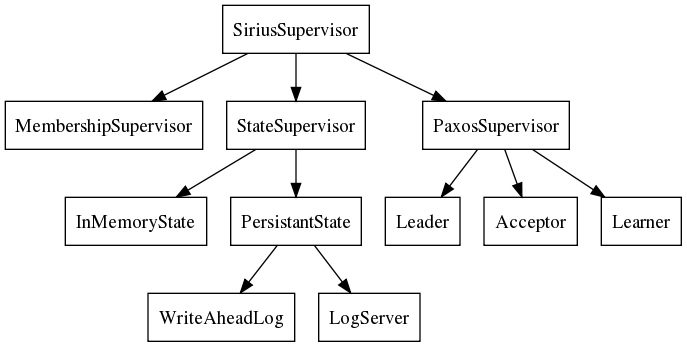
\includegraphics{img/actor_hierarchy.png}}

\subsubsection{Sirius Supervisor}

\subsection{Initialization}

%%-------------------------
%% Write Ahead Log Format
%%-------------------------
\section{Write Ahead Log Format (UberStore)}

%%------------------------------
%% Write Ahead Log Format:
%%    Principles of Some Import
%%------------------------------
\subsection{Principles of Some Import}
The Sirius write-ahead log was initially designed with the goals of replayability,
compactability, and human readability in mind. However, over time, performance demands
came to reveal that a human readable format and efficient query operations over the
log were at odds with each other.  Therefore, the human readable goal was forgone
in favor of efficiency.

The goals of the Sirius write-ahead log, endearingly termed "UberStore" in its redesign,
are now the following:

\begin{itemize}
\item {\em Replayability-} 
    Iterating over all of the events in the log, in strict order, 
    should be possible and efficient.
\item {\em Compactability-}
    Receiving an unbounded stream of events the write-ahead log
    may grow without bound. With the observation that any event
    in the log may nullify some set of previous events, there must
    be a way to transform a log to a format in which those nullified
    events are removed. This provides a means for bounding log growth.
\item {\em Efficient Random Access-}
    It must be possible to efficiently select an arbitrary subrange of
    events from a log.
\end{itemize}

Efficient Random Access was the major driver of the log redesign.


%%------------------------------
%% Write Ahead Log Format:
%%    Design Overview
%%------------------------------
\subsection{Design Overview}
The Sirius write-ahead log format, UberStore, is an append only store largely influenced
by Basho's BitCask\footnote{http://downloads.basho.com/papers/bitcask-intro.pdf} and
Facebook's Haystack\footnote{http://www.facebook.com/note.php?note\_id=76191543919}.

Entries are appended to one file, and sequence number to offset mappings are stored
in a separate file. We refer to these as the {\em data} and {\em index} files. Both files
are encoded in a binary format using the FNV-1a\footnote{http://en.wikipedia.org/wiki/Fowler\%E2\%80\%93Noll\%E2\%80\%93Vo\_hash\_function}
checksum algorithm, chosen for its speed and simplicity.

\subsection{UberStore}
Data and Index Files are associated by their file name.  The naming convention for them
is the first sequence number contained in the pair with the extension "data" for a
Data File and "index" for an Index File.

\subsection{Data File}
The Data File is append-only; all written data is immutable.  Data is stored in a binary
format with numeric types encoded in big-endian byte-order. For the following {\em int}s
are signed and 4 bytes, and {\em long}s are signed and 8 bytes.

The base entry format is as follows:

\begin{center}
    [length: int][checksum: long][payload: ...]
\end{center}

The {\em length} field contains the length of the {\em payload} field. The
{\em checksum} field only covers the {\em payload} field- if the length
field is corrupted then the checksum will not cover the proper bytes, and therefore
the checksum check will fail, indicating corruption.

The payload field is an arbitrary array of bytes. This field currently encapsulates
ordered events from Sirius, which are encoded as follows:

\begin{center}
    [seq: long][timestamp: long][type: int][keyLen: int][bodyLen: long][key: ...][body: ...]
\end{center}

The {\em type} field is an encoding of the event type, either 1 for {\em Put} or 2 for
{\em Delete}.  The {\em keyLen} bytes immediately following the {\em bodyLen} contain the key.
The {\em bodyLen} bytes following the key contain the event body. Note that for {\em Delete}
this is empty.

\subsection{Index File}
Similar to the Data File, the Index File is append only and all written data is
immutable. The index contains {\em long}s (signed, 8 bytes) in sets of 3. The entry
format is as follows:

\begin{center}
    [checksum: long][sequenceNumber: long][offset: long]
\end{center}

The {\em checksum} field covers the entire entry, with the checksum field set to 0.
The rest of the entry is reasonably direct, {\em sequenceNumber} is found at offset
{\em offset} in the associated Data File.

\subsection{Data/Index Interaction}
All writes go first to the Data File, and then are written into the Index File.
We enforce the invariant that the files are totally ordered by sequence number
by only allowing events to be written in strictly increasing sequence number order.
Gaps, however, are tolerated.

Read operations are based on sequence number range. The Index File is first consulted
for the appropriate offset range to query in the Data File.  Then, querying the range
is as simple as seeking to the first offset and decoding entries until the end of the
range.  This methodology has the indirect benefit of preventing us from attempting to
read incomplete entries as they are written, providing some thread safety.

For performance, the Index File's contents are cached, and the only reason to hit disk
for the Index File is to write a new offset.

\subsection{Corruption Recovery}
When dealing with the filesystem and multiple files, there is some possibility of
corruption. UberLog does its best to make it easy to recover from these types of
corruption. Following are the possible failure scenarios, how UberStore handles them,
and what human intervention, if any, is required.

\subsubsection{Missing Index File}
UberStore will gracefully recover from a missing Index File by reading the entire associated
Data File and generating a new one.

\subsubsection{Incomplete Index File}
The Index File may be incomplete if a write makes it into the Data File but not the Index
File. The most likely source of this is that the host system shuts down after the Data
File has been written to, but before the Index File could be. UberStore will gracefully
recover from this situation by seeking to the last event known by the Index File, and
updating the Index File with all events from that point.

\subsubsection{Corruped Index File}
Simply delete the Index File and allow the {\em Missing Index File} recovery kick in.

\subsubsection{Corrupted Data File}
Not all data can be recovered, but all data up to the corruption point may be recovered
by truncating at the point of corruption. Then remove the Index File and allow it to
regenerate.

\subsubsection{Missing Data File}
This is bad, if you're missing a Data File there's no recovery, because that's how it works.

\subsection{Compaction Algorithm}
The write-ahead log may grow indefinitely in size. Therefore, it is necessary to bound this
growth to the best degree possible.

Using the observation that {\em Put}s and {\em Delete}s for a given key cancel each
other, out this is reasonably simple and only involves retaining the last {\em Put}
or {\em Delete} in a log for a given key. Once these have been selected we simply
write them out to a new log in the order in which they appeared in the original
log.

%%------------------------------
%% Cluster Membership:
%%    Join Algorithm
%%------------------------------
\section{Cluster Membership}
Cluster membership is maintained by the membership subsystem.  It is this subsystems responsibility for maintaining the Set of all members in the cluster.  This membership is stored in a shared area and is accessible to all local subsystems.  It is an unwritten rule that only the membership subsystem is allowed to modify membership.

\subsection{Implementation}
Membership is stored in a file which is polled by the membership subsystem. This file contains the Actor Address\footnote{http://doc.akka.io/docs/akka/snapshot/general/addressing.html} of each of the cluster members on new lines.

\end{document}
